\subsection{Product description}
\label{sec:product-desc}

% What kind of product
An automotive \gls{asic} was tested for highlighting a practical case of functional failure.
The studied chip performs several high-level and critical functions for the car vehicle.

% What kind of failure
The failure was discovered while putting the chip in a lowered configuration.
In this configuration, the amount of external devices was reduced.
The goal is to check if the robustness of the chip against \gls{esd}s is impacted.

With the normal configuration, the failure \textbf{never} happens (up to the maximum testing limit).
Failures happen only with the lowered configuration.
As a side note, the lowered configuration is relevant because the \gls{bom} of the system is smaller, and manufacturing costs are reduced.

\begin{figure}[!htbp]
  \centering
  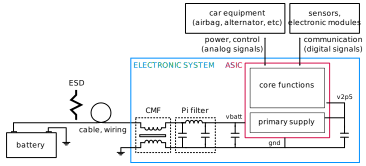
\includegraphics[width=0.9\textwidth]{src/3/figures/architecture_system.pdf}
  \caption{Overview of the system architecture}
  \label{fig:system_architecture}
\end{figure}

% Difference of configs
The input used during the tests to inject the \gls{esd} inside the system is the battery supply connection (Fig. \ref{fig:system_architecture}).
The normal configuration uses strong differential and common-mode filtering on this input.
This technique very effectively deviates the stress current into a ground before it even has a chance to reach the chip under test.
In the lowered configuration, only a reduced differential filtering is present on the input.

% What is being tested
Inside the \gls{ic}, the study focuses on the primary supply function (Fig. \ref{fig:monitored_function}).
This function is the first to start when the chip is powered-on.
It powers many blocks, especially sensitive digital cells and low-voltage analog functions.

% Why testing this function
There are two motivations for testing this particular function.
One of its input (battery input) is an external pin and is also exposed as the system level.
This pin can very likely be exposed to electrostatic discharges during real operation.
Then, one of its output is also exposed externally, because the function requires a large capacitor for stabilisation that cannot be integrated on silicon.
This pin is a very convenient monitoring point during tests.

%TODO: Increase font size
\begin{figure}[!htbp]
  \centering
  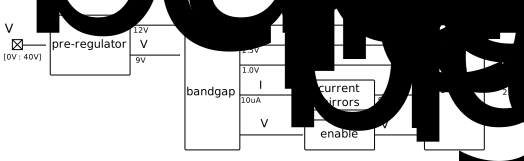
\includegraphics[width=0.9\textwidth]{src/3/figures/monitored_function.pdf}
  \caption{Architecture of the primary supply}
  \label{fig:monitored_function}
\end{figure}


\subsubsection{Integrated supply function description}

% Main task
The main function of the regulation function is to down-convert a battery voltage to a 2.5V regulated supply.
Several blocks are involved for processing the battery supply.
The overall architecture is given in fig. \ref{fig:monitored_function}).

%TODO: Uniform net names
% First block
First, a pre-regulator clamps the battery voltage that can reach up to 40V down to 9V.
This is done to protect more sensitive circuitry connected downstream.
This output has low current capability and is used for low-power functions.
A second output provides a 12V clamped output with a large current capability.

% Second block
A bandgap reference is connected downstream.
It is powered by the 9V supply.
Once properly started after a certain delay, the bandgap generates a 1.0 V voltage reference.
This reference is stable accross a wide range of temperature, process variation and process mismatchs.
The bandgap also outputs a 10uA current reference, and a flag \textit{bgok} to signal it is ready for operation.

% Third major block
Finally, the \gls{ldo} regulator generates a stable 2.5V supply voltage, able to deliver and sustain up to 20mA.
In the original product, this output is used further in the system to power digital gates.

% Detail nets connections
The regulator relies on multiple signals generated in the upstream blocks for operation.
The most critical nets are the 1.0V reference from the bandgap, and the ramp-up signal.
Circuit analysis show that both nets can directly affect the output voltage.
A variation on the reference voltage is immediately copied on the output.
The ramp-up signal controls the soft-start of the regulator, that can directly change the output value.
Other nets provide bias to the regulator, and their impact on the output is more limited.

% Talk about external devices
The regulator is connected externally to a 100nF decoupling capacitor to absorb peak currents and achieve stability.

% What are the minor blocks doing
The \textit{current mirrors} provide copied current values from the bandgap, while offering much larger output impedance.
The \textit{enable} block mostly checks and waits for the bandgap to be properly started.
It then triggers a startup ramp-up sequence on the regulator.
